% Number 520
% BFPM SFriction Vectors Algebra Units Tension
% Balanced forces - multiple ropes, static friction
% KO

% Watermark
\AddToShipoutPicture*{\BackgroundPic}

\addtocounter {ProbNum} {1}

\begin{floatingfigure}[r]{.45\textwidth}
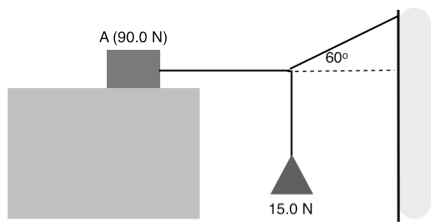
\includegraphics[scale=.6]{/Users/jgates/desktop/latex/pics/static1}
\end{floatingfigure}
 
{\bf \Large{\arabic{ProbNum}}} In the diagram, there is a block (Block A) with weight 90.0 N resting on the table. The coefficient of static friction between the block and the surface on which it rests is 0.30. Block A is connected to a hanging mass with weight 15.0 N. The hanging mass is also connected to the wall, with the angle of the connecting string being 60 degrees.

\bigskip
Determine the force of friction that must be acting on Block A if the entire system is at rest.
\paragraph{}
\noindent
\vfill
Determine the maximum weight that the hanging mass may have, if all other conditions stay the same.

%\hfill 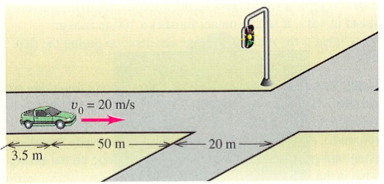
\includegraphics[scale=.85]{/Users/jgates/desktop/latex/pics/redlight.png}


\vfill
\newpage
